\chapter{Implementación}
En el capítulo anterior se explicó la teoría necesaria para entender las propiedades físicas de un quadcopter así como el algoritmo SLAM para explicar como se lleva acabo la autonomía en los robots móviles. Si bien cada caso del proceso total podría ser implementarse desde cero, se ha optado por hacer uso de las librerías especializados en robótica que se encuentra en ROS.

En esta sección se explicará sobre el sistema operativo para robots (ROS), luego se describirá los componentes del quadcopter que se va a utilizar para este proyecto, posteriormente se explicará sobre el sensor láser y el controlador de vuelo Pixhawk. Finalmente se explicará sobre el software que se realizó para realizar la autonomía del quadcopter y los mapas tridimensionales.

\section{Robot Operating System (ROS)}
ROS es un framework que se usa ampliamente en robótica. Lo que busca este sistema operativo de código abierto es hacer una pieza de software que pueda funcionar en otros robots con solo pequeños cambios en el código. Lo que obtenemos con esta idea es la capacidad de crear funcionalidades que se pueden compartir y usar en otros robots, por lo que no necesitamos volver a reinventar la rueda.

ROS fue desarrollado originalmente en el 2007 por el laboratorio de Inteligencia Artificial de Stanford (\textit{SAIL}) en apoyo del proyecto Stanford AI Robot \cite{rosHistory}. A partir del 2008, el desarrollo continúa principalmente en Willow Garage, un instituto de Investigación de Robótica, con más de veinte instituciones colaborando dentro de un modelo de desarrollo federado.

Muchas instituciones de investigación han comenzado a desarrollarse en ROS, agregando hardware y compartiendo su código. Los sensores y actuadores utilizados en la robótica también se han adaptado para su uso en ROS. Gracias a esto, las empresas están creando sensores más baratos y más potentes. Arduino es un buen ejemplo de esto, ya que al usar una placa electrónica barata puede agregar una gran cantidad de sensores como codificadores, sensores de luz, temperatura, y así sucesivamente \cite{rosIntroduction}.

ROS proporciona las instalaciones del sistema operativo estándar, como la abstracción de hardware, el control de dispositivos de bajo nivel, la implementación de funcionalidades de uso común, el paso de mensajes entre procesos y la gestión de paquetes. Esta tesis es desarollada con librerías de ROS.

\section{Hardware usado}
En esta sección se explicará los componentes que se utilizó para realizar el proyecto. Se comenzará describiendo el quadcopter, posteriormente el sensor láser que fue utilizado, el microcontrolador donde fue implementado el algoritmo SLAM y finalmente del controlador de vuelo Pixhawk.

\subsection{Fantom}
Fantom es el quadcopter que fue desarrollado en el laboratorio de robótica de la Universidad de Ingeniería y Tecnología - UTEC, en el año 2015 (Figura \ref{f:fantom}). Este drone fue construído de forma experimental utilizando los motores del DJI Phantom 2; tiene un peso de aproximadamente 1100 gramos (incluyendo batería) y puede cargar 1000 gramos más según las características de sus motores y las pruebas realizadas en el laboratorio. Fantom fue construído para fines aplicativos orientado a métodos de control no lineal.Este drone esta compuesto por:

\begin{itemize}
\item[•] Quadcopter Frame fibra de vidrio de 480 mm.
\item[•] Multi-Rotor Lipo 4S de 4000 mAh.
\item[•] Multi-Rotor ESC 4S ~ 6S de 20 A.
\item[•] Motores Brushless 960KV.
\item[•] Controlador de vuelo Pixhawk.
\end{itemize}
%\begin{figure}[htb]
%\centering
%\subfloat[Original Image]{\includegraphics[width=40mm]{frame.jpg}}
%~\subfloat[Edges using Canny]{\includegraphics[width=40mm]{bateria.jpg}}\\
%~\subfloat[Dilate Image]{\includegraphics[width=40mm]{dilation_taza.jpg}}
%\subfloat[Morphologically closed image]{\includegraphics[width=40mm]{ESC.jpg}}
%~\subfloat[Skeletonized image]{\includegraphics[width=40mm]{motor.jpg}}
%\subfloat[Morphologically closed image]{\includegraphics[width=40mm]{pixhawk.jpg}}
%\caption{Image processing steps for a 3D real scene} \label{f:cup}
%\end{figure}
\begin{figure}
\centering
\includegraphics[scale=0.1]{fantom.jpg}
\caption{Quadcopter Fantom.}
\label{f:fantom}
\end{figure}

\subsection{RPLIDAR A2}
Es un sensor láser que se basa en el  principio de rango de triangulación láser \cite{amann2001laser} y adopta el hardware de adquisición y procesamiento de visión de alta velocidad desarrollado por \textit{SLAMTEC}. El sensor utiliza un láser infrarrojo de baja potencia como su fuente de luz y lo maneja utilizando un pulso modulado.Este sensor gira a 360 \grad ~y llega a una distancia máxima de 8 metros. Trabaja a una frecuencia de 10 Hz y tiene una tasa de medición de 4000 muestras por segundo. El hardware del RPLIDAR A2 se puede ver en la figura \ref{f:lidar}, el cual tiene un convertidor de protocolo UART a mini USB.
\begin{figure}
\centering
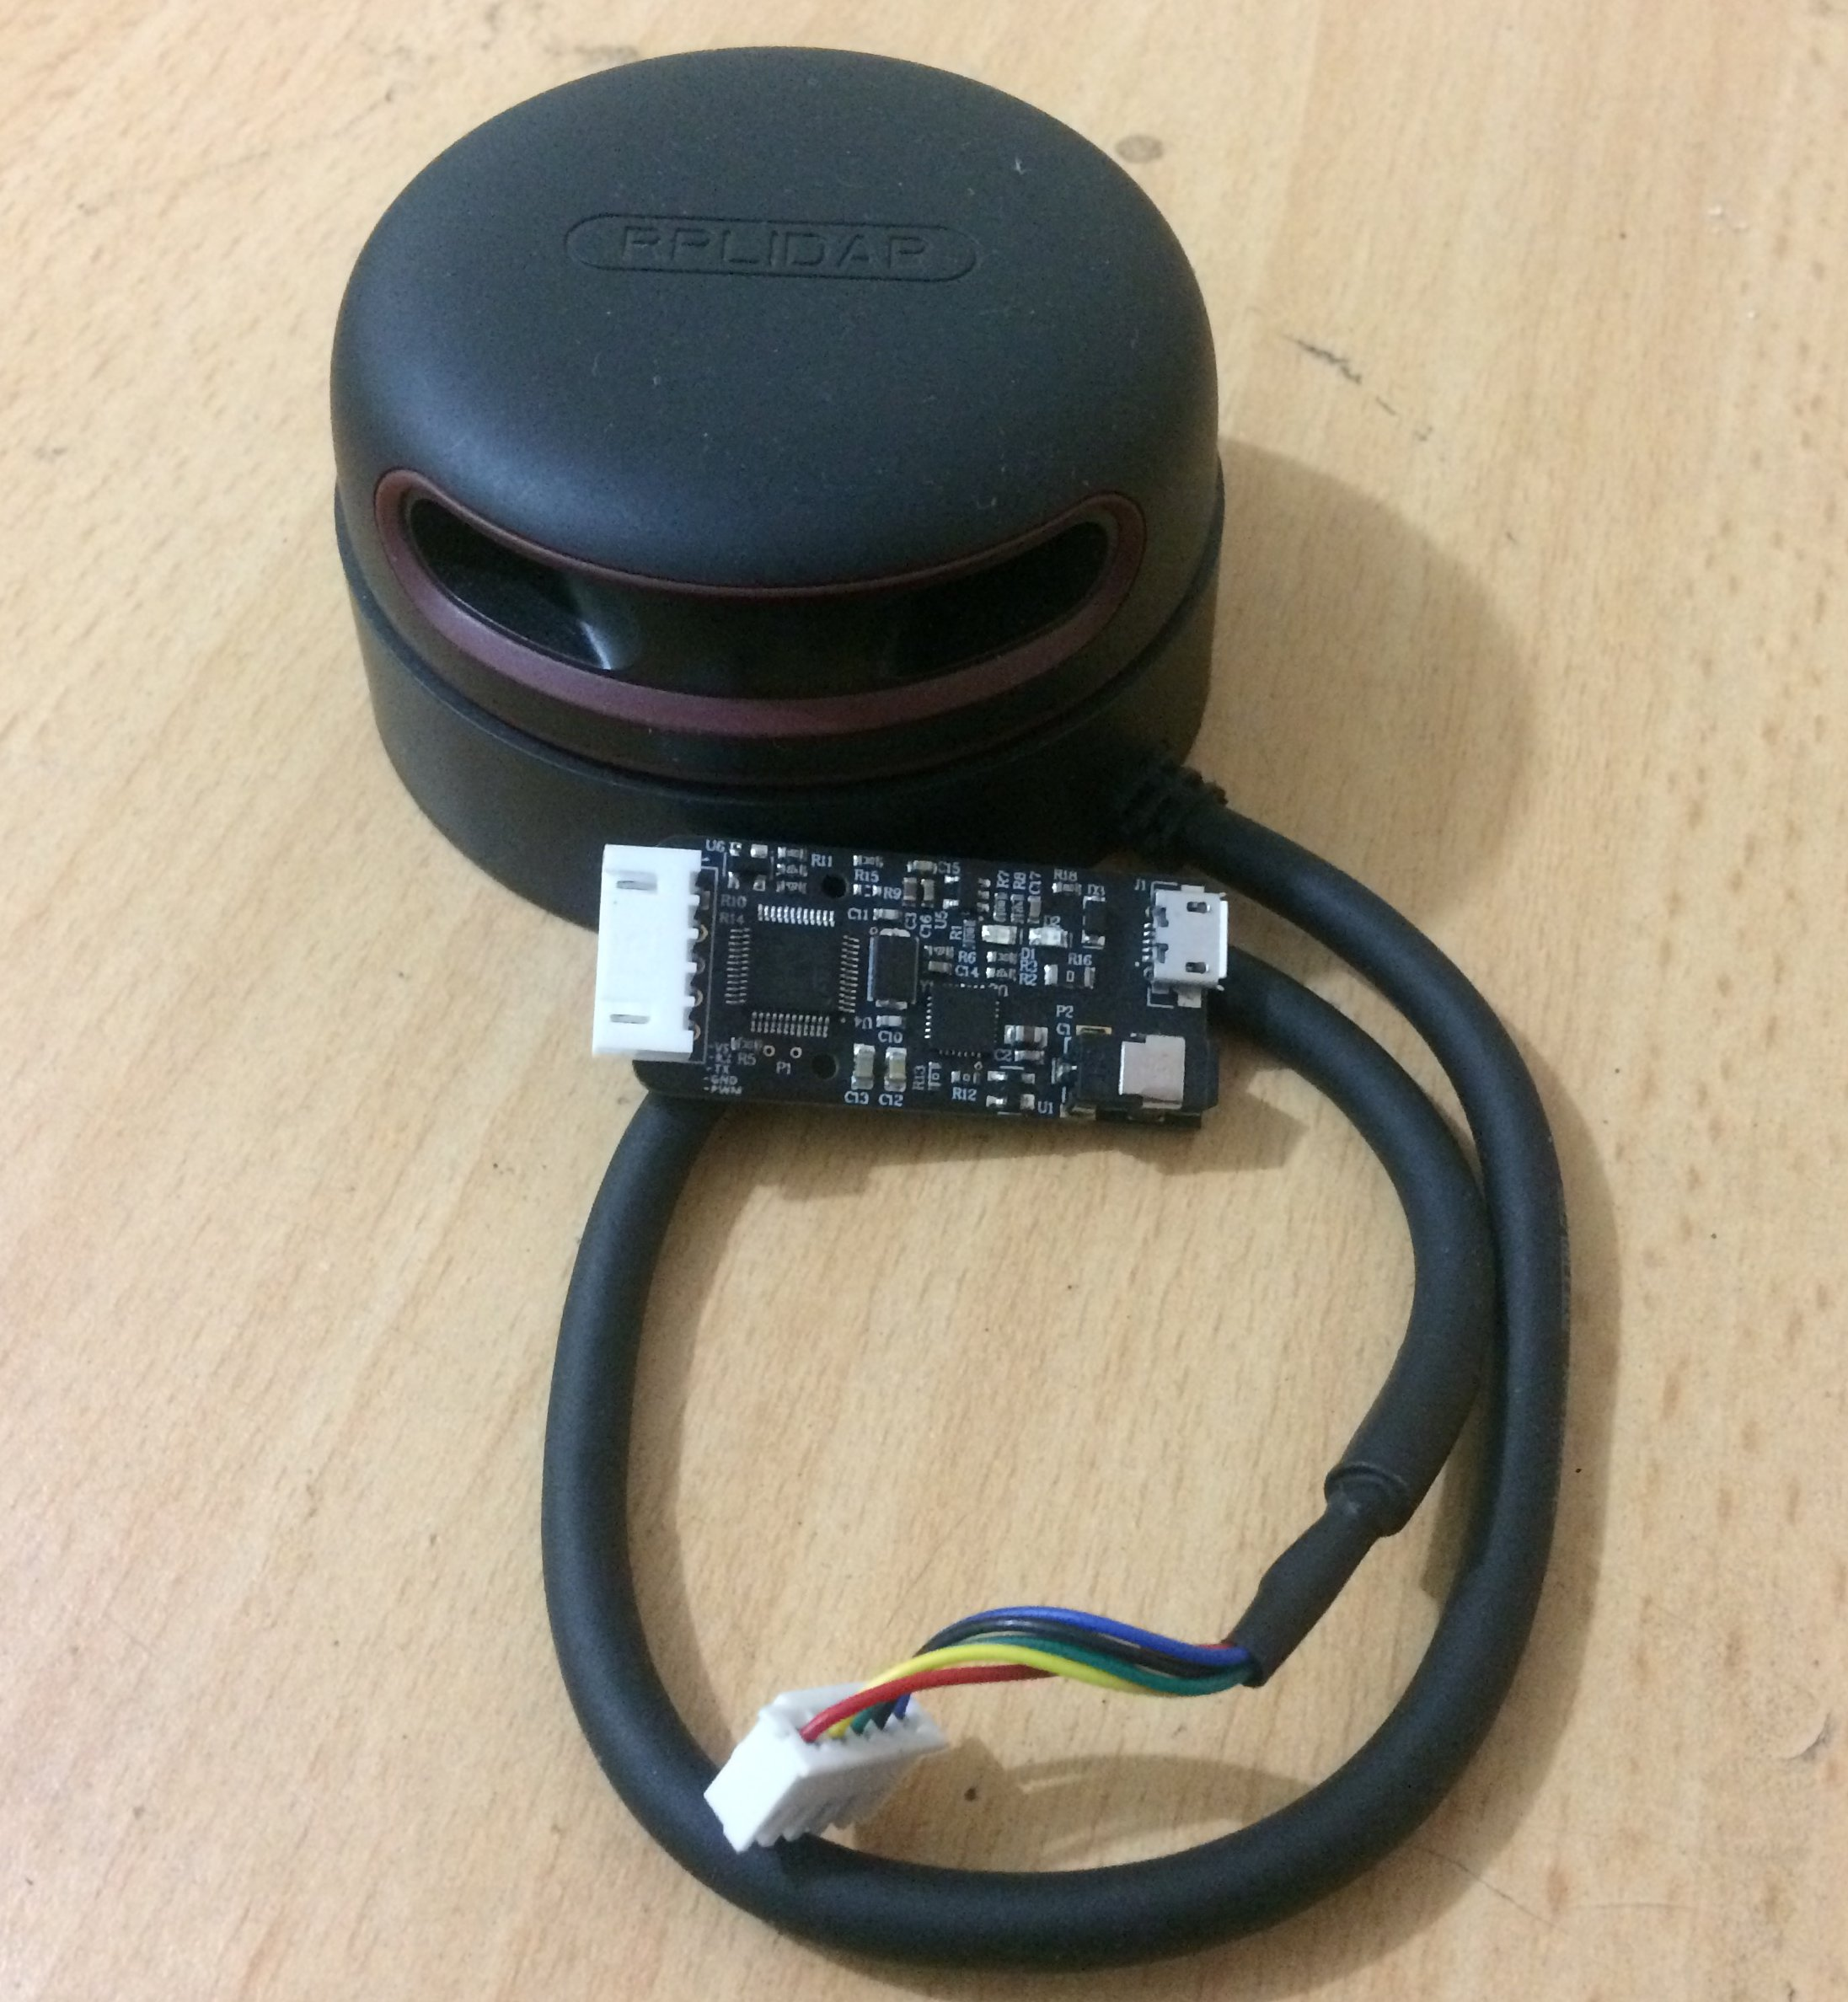
\includegraphics[scale=0.1]{rplidar.JPG}
\caption{Sensor láser RPLIDAR A2.}
\label{f:lidar}
\end{figure}


\begin{table}[htbp]
\begin{center}
\begin{tabular}{|l|c|c|c|c|}
\hline
Item & Unidad & Mínimo & Típico & Máximo\\
\hline \hline
Rango de distancia & m & 0.15 & - & 8 \\ \hline
Rango angular & grados & - & 0 - 360 & - \\ \hline
Resolución de la distancia & mm & - & menor a 0.5 & - \\ \hline
Duración de muestra & ms & - & 0.25 & - \\ \hline
Resolución angular & grados & 0.45 & 0.9 & 1.35 \\ \hline
Fecuencia de muestreo & Hz & 2000 & 4000 & 4100 \\ \hline
Frecuencia de escaneo & Hz & 5 & 10 & 15 \\ \hline
\end{tabular}
\caption{Pruebas de Medición.}
\label{tbl:medicion}
\end{center}
\end{table}

La tabla \ref{tbl:medicion} muestra el rendimiento de medición \cite{Slamtec} que tiene el sensor láser considerando varias pruebas por cada item. Este sensor tiene una interfaz de comunicación (UART) el cual esta dividido por pines y colores de cables esto se muestra en la tabla \ref{tbl:comunicacion}. Por medio de este protocolo se controla el motor (PWM) y los datos que el sensor envía a una PC o microcontrolador. El RPLIDAR A2 envía los datos después de recibir una solicitud de un sistema host, una vez que el sensor reciba esta solicitud enviará los datos del escaneo de forma continua al sistema host.

\begin{table}[htbp]
\begin{center}
\begin{tabular}{|c|c|c|c|c|c|}
\hline
Color & Nombre de la señal & Tipo & Mínimo & Tipico & Máximo \\ 
\hline \hline
Rojo & VCC & Potencia & 4.9V & 5V & 5.5V \\ \hline
Amarillo & Tx & Salida & 0V & 3.3V & 3.5V \\ \hline
Verde & Rx & Entrada & 0V & 3.3V & 3.5V \\ \hline
Negro & GND & Potencia & 0V & 0V & 0V \\ \hline
Azul & MOTOCTL & Entrada & 0V & 3.3V & 5V \\ \hline
\end{tabular}
\caption{Interfaz de comunicación del sensor láser.}
\label{tbl:comunicacion}
\end{center}
\end{table}

\subsection{Sensor IMU}
El controlador de vuelo consta de un sensor IMU (acelerómetro, giroscopio y magnetómetro). InvenSense MPU6000 es el sensor IMU y ST Micro L3GD20H + LSM303D o InvenSense ICM2076 actúan como sensores de respaldo \cite{pixhawkIMU}. El primer conjunto de sensores se coloca en la placa primaria de la FCU mientras que el tercer conjunto se coloca en la placa aislada de las vibraciones. Las lecturas de estos diferentes conjuntos de sensores se colocan en buses separados. Son responsables de proporcionar la medición inercial necesaria para maniobrar el quadcopter. Las lecturas del giroscopio que indican la rotación de las aeronaves sobre sus propios ejes son necesarias para un vuelo estable, utilizado internamente por el controlador PID. Las lecturas del acelerómetro proporcionan las fuerzas de aceleración y aceleración en los 3 ejes, ayudan en el control de la posición de la aeronave. Esta información se puede utilizar para la estimación de la posición, pero se sabe que es propensa a errores. El magnetómetro o la brújula es responsable de proporcionar información sobre el campo magnético de la tierra e inferir el norte magnético.

\subsection{Sensor Barométrico}
El controlador de vuelo consta de 2 sensores barométricos MS5611 redundantes. Mide la presión del aire y, en teoría, se puede utilizar para predecir la altitud, pero necesita una recalibración frecuente.
 
\subsection{Controlador de Vuelo}
Pixhawk \cite{PixhawkHome}, fabricado por Proficnc es la unidad de controlador de vuelo a bordo del quadcopter que vamos a utilizar en este proyecto (Figura \ref{f:pixhawk}). La función de este dispositivo es leer los datos de entrada de los sensores (láser e IMU), realizar cálculos y, como resultado, manipular la velocidad de los motores para ejecutar las manibras necesarias. Es un piloto automático de código abierto donde los desarrolladores se encargan de compartir en los repositorios de Ardupilot \cite{Ardupilot}. Para mejorar las lecturas del sensor IMU, el Pixhawk viene con 3 sistemas IMU redundantes, que están aislados entre sí, y también están amortiguados para evitar que las vibraciones del vuelo corrompan los datos.

El Pixhawk viene con un IMU desacoplado y FMU (unidad de gestión de vuelo) para reducir la interferencia a los sensores. Tiene un núcleo ARM Cortex M4 de 32 bits con FPU que opera a una frecuencia de 168 Mhz, 256 KB RAM, memoria flash de 2 MB y un coprocesador a prueba de fallos de 32 bits (REFERENCIAR DATASHEET). Los sensores a bordo se discute a detalle en las subsecciones 3.2.3 y 3.2.4.
El Pixhawk viene con un solo suministro independiente de 5V para el controlador de vuelo y sus periféricos. También proporciona protección contra sobre voltaje, protección contra sobrecorriente y protección térmica. La FMU y la IO (entradas y salidas) funcionan a 3.3V y 6.6V. Se puede alimentar a través de USB o a través de los 2 conectores. Para las operaciones IO, viene con un puerto I2C, 2 puertos CAN, 5 puertos UART, un puerto SPI y un puerto RSSI (PWM o Voltaje).

\begin{figure}
\centering
\includegraphics[scale=0.4]{pixhawk.jpg}
\caption{Controlador de Vuelo Pixhawk}
\label{f:pixhawk}
\end{figure}

%\section{Arquitectura de Solución}
%\subsection{Arquitectura del Sistema}
%\subsection{HectorSlam}
%\subsection{Mavros}

